\chapter{Realisieren}
In diesem Kapitel geht es um die Implementation der Software. Diese richted sich nach den Diagrammen aus dem Kapitel
\ref{chap:plan}, Planen.

\section{Entwicklungsumgebung}
\subsection{Versionierung}
Für die Versionierung wird Git verwendet. Dabei wird GitHub als Remote-Repository verwendet. Das Repository mit
dem Source-Code kann unter \url{https://github.com/aneshodza/gnosis} gefunden werden. Für eine genauere Beschreibung
der Versionierung siehe Kapitel \ref{sec:versioning}.
\subsection{IDE}
Als IDE wird vim mit verschiedenen Plugins verwendet. Bestimmte Sachen wurden in der \bgmintinline{bash}{.vimrc} Datei
konfiguriert, damit die Arbeit möglichst effizient ist. \newline
Diese Konfigurationen sind unter \newline
\url{https://github.com/aneshodza/.dotfiles/blob/ad87ee9ecc5588a59d66e211797792099569ca95/.vimrc} zu finden.
\subsection{CI/CD}
Für die CI/CD Pipeline wird SemaphoreCI verwendet. Das ist passend, da auch die PA sehr eng mit SemaphoreCI verbunden
ist.

\section{Aufsetzen des Projektes}
Zu Beginn wird Arbeitspaket 7, Aufsetzen des Projektes, implementiert. Dazu sind folgende Schritte zu befolgen:
\begin{enumerate}
  \item Erstellen des Plugins
  \item Erstellen des Remote-Repository
  \item Mit dem README beginnen
  \item Aufsetzen der CI/CD Pipeline
\end{enumerate}

\subsection{Erstellen des Plugins}
Um das Plugin aufzusetzen begeben wir uns in das Verzeichnis der Lokalen Redmine Instanz. Diese wurde in den
Vorarbeiten bereits erstellt und aufgesetzt. \newline
Dort wird mit dem Befehl \bgmintinline{bash}{bundle exec rake generate redmine_plugin gnosis} das Plugin erstellt. Der
Konsolen-Output sieht wie folgt aus:
\begin{codebox}[]
  \begin{minted}{bash}
> bundle exec rails generate redmine_plugin gnosis
create  plugins/gnosis/app
# Lots of things being created...
create  plugins/gnosis/README.rdoc
# Lots of things being created...
create  plugins/gnosis/test/test_helper.rb
  \end{minted}
\end{codebox}

Wenn wir dann mit \bgmintinline{bash}{cd plugins/gnosis} in das Plugin wechseln, sehen wir, dass bestimmte Dateien
bereits erstellt wurden. Diese werden bei Gebrauch erklärt und aufgezeigt.

\subsection{Erstellen \& Konfigurieren des Repository}
Das Projekt wird auf GitHub mit Git Versionsverwaltet, weshalb als Erstes ein GitHub Remote-Repository (auch einfach
Repository genannt) erstellt werden muss. Das wird nach GitHub Dokumentation gemacht \cite{github_create_repo}.

\subsubsection{Erstellen des Lokalen Repostiory}
Danach muss das lokale Plugin mit dem Repository verbunden werden. Dazu müssen wir mit der Konsole in das Directory
unseres Plugin wechseln, welches unter \menu{redmine/plugins/gnosis} zu finden ist. \newline
Dort initialisieren wir das lokale Repository mit \bgmintinline{bash}{git init} und verbinden es mit dem Remote
Repository indem wir \bgmintinline{bash}{git remote add origin [URL]} ausführen.

\subsubsection{Initial Commit}
Nun können wir den ersten Commit machen. Das können wir ganz einfach mit wenigen Befehlen machen:
\begin{codebox}[]
  \begin{minted}{bash}
> git add -A
> git commit -m "Initial commit"
> git push -u origin main
  \end{minted}
\end{codebox}

\subsubsection{Git-flow initialisieren}
Das Projekt wird nach der Git-flow Methode versioniert. Das bedeutet, dass der main Branch für die Releases
verwendet wird und der develop Branch für die Entwicklung. \newline
Dafür müssen wir den develop branch mit \bgmintinline{bash}{git checkout -b develop} erstellen und diesen
mit \bgmintinline{bash}{git push -u origin develop} auf remote pushen. \newline

\subsection{Erstellen des README}
Beim Erstellen des Plugins wurde automatisch ein \enquote{README.rdoc} erstellt. Dieses wird bei Ruby Projekten
oft anstatt eines \enquote{README.md} verwendet. Da diese PA nach Vorgaben von Redmine arbeitet, wird auch ein
README im rdoc Format geschrieben. Es wird auch eins im README Format geschrieben, welches mehr ausführt, da dieses
bereits beim öffnen des Repositores auf GitHub sichtbar ist. \newline
Da noch nicht viel im Projekt steht, wird nur beschrieben was genau das Plugin kann und wie es funktioniert.

\subsection{Aufsetzen der CI/CD Pipeline}
Die CI/CD wird auf SemaphoreCI eingerichtet, weshalb wir uns dort anmelden und ein neues Projekt erstellen. Man kann dieses
direkt mit GitHub verbinden und Semaphore die meiste Arbeit machen lassen.

\subsubsection{Erstellen der \enquote{bin files}}
Da die Tests sowie Linter immer wieder ausgeführt werden, ist es sinnvoll diesen Prozess zu automatisieren. Dazu werden 
\enquote{bin files} erstellt. Diese sind kleine Bash-Scripts, welche repeditive Aufgaben automatisieren. In unserem Fall sind
das die Ausführungen von den Tests und Lintern sowie das aufsetzen des Projektes. \newline

Für die Tests wird ein \bgmintinline{bash}{bin/test} mit folgendem Inhalt erstellt:
\begin{codebox}[]
  \begin{minted}{bash}
#!/bin/bash

white='\033[1;37m'
red='\033[0;31m'
green='\033[0;32m'

rake redmine:plugins:test

if [[ $? -eq 0 ]]; then
  echo -e "${green}----------------------------------------"
  echo -e "Tests passed"
  echo -e "----------------------------------------${white}"
else
  echo -e "${red}----------------------------------------"
  echo -e "Tests failed"
  echo -e "----------------------------------------${white}"
  exit 1
fi
  \end{minted}
\end{codebox}

Dann braucht es ein \bgmintinline{bash}{bin/fastcheck} für linter und so weiter mit folgendem Inhalt:
\begin{codebox}[]
  \begin{minted}{bash}
#!/bin/bash

white='\033[1;37m'
red='\033[0;31m'
green='\033[0;32m'

function return_code {
if [ $? -ne 0 ]; then
  echo -e "${red} Error: $1 found errors! ${white}"
  failing_checks+=("$1")
  passing=false
fi
}

passing=true
failing_checks=()

echo "Executing fastchecks..."

if [[ $* == *--fix* ]]; then
echo "Fixing..."
bundle exec rubocop -a --config .rubocop.yml
return_code "Rubocop"
else 
echo "Note: You can use --fix to fix the errors automatically"
bundle exec rubocop --config .rubocop.yml
return_code "Rubocop"
fi

bundle exec brakeman -q -z --no-summary --no-pager
return_code "Brakeman"

if [ "$passing" = true ]; then
echo -e "${green}----------------------------------------"
echo -e "All checks passed"
echo -e "----------------------------------------${white}"
exit 0
else
echo -e "${red}----------------------------------------"
echo -e "Some checks failed"
echo -e "Failed checks: ${failing_checks[@]}"
echo -e "----------------------------------------${white}"
exit 1
fi
  \end{minted}
\end{codebox}

Dann braucht es ein \bgmintinline{bash}{bin/setup} für das aufsetzen des Projektes mit folgendem Inhalt:
\begin{codebox}[]
  \begin{minted}{bash}
yarn install
bundle exec rake redmine:plugins:migrate
  \end{minted}
\end{codebox}

\subsubsection{Erstellen der \enquote{semaphore.yml} Datei}
Was wir noch machen müssen, ist die \bgmintinline{bash}{semaphore.yml} Datei zu erstellen. Diese muss ungefähr folgenden Ablauf
ausführen:
\begin{enumerate}
\item Redmine klonen und Aufsetzen
\item Postgres starten
\item Datenbank erstellen und migrieren
\item In das Plugins directory wechseln
\item Plugin klonen
\item Tests ausführen
\end{enumerate}

Auf einem Activity Diagramm würde das so aussehen:
\begin{figure}[H]
  \centering
  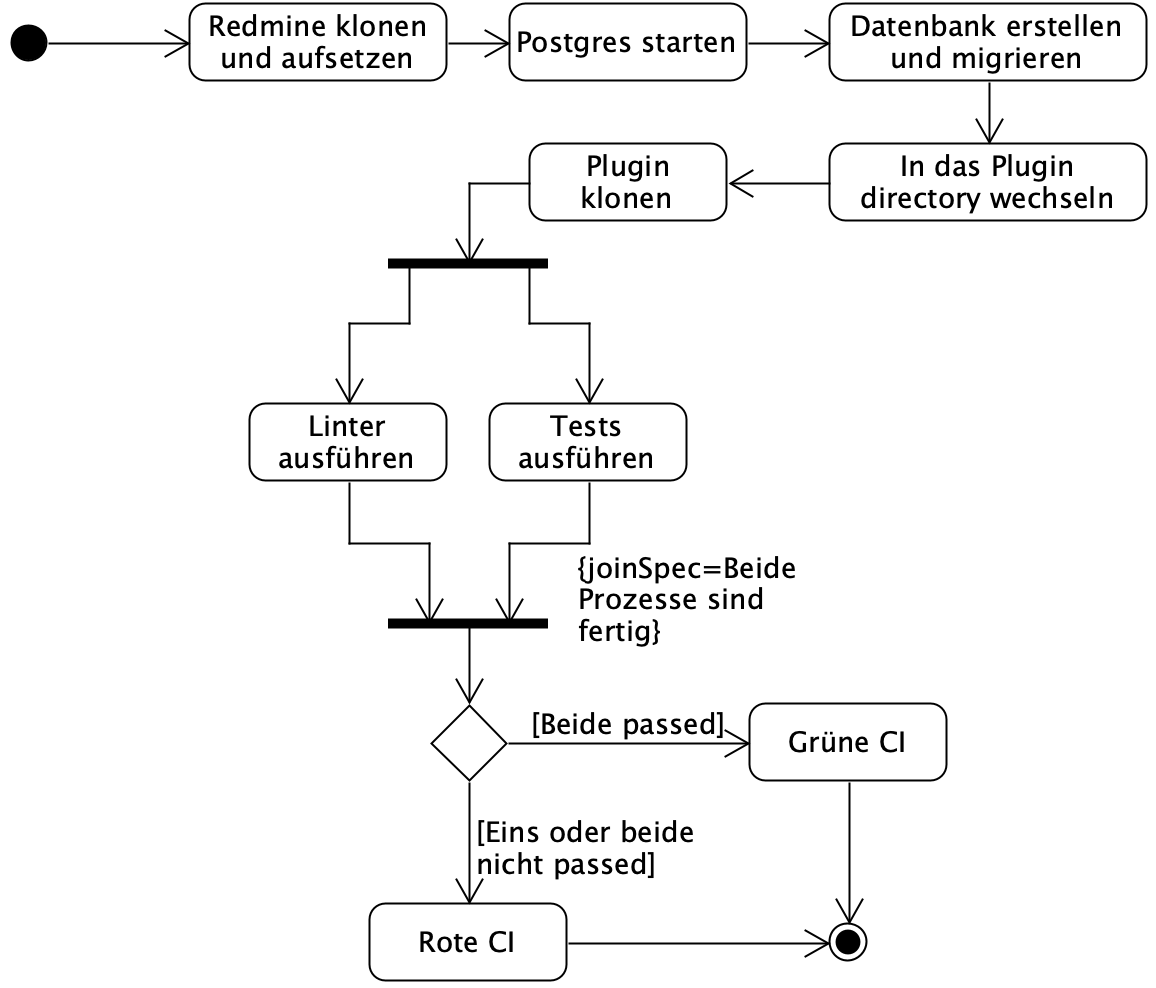
\includegraphics[width=0.8\textwidth]{images/activity/ci-cd.png}
  \caption[Activity Diagramm der CI/CD Pipeline]{Activity Diagramm der CI/CD Pipeline}
  \label{fig:activity_ci_cd}
\end{figure}

Die oben beschriebene semaphore.yml Datei sieht dann so aus:
\begin{codebox}[]
  \begin{minted}{yaml}
version: v1.0
name: Initial Pipeline
agent:
machine:
  type: e1-standard-2
  os_image: ubuntu2004
blocks:
- name: Checks
  task:
    jobs:
      - name: Tests
        commands:
          - bin/test
      - name: Linter
        commands:
          - bin/fastcheck
    prologue:
      commands:
        - 'git clone git@github.com:redmine/redmine.git'
        - cd redmine
        - cp config/configuration.yml.example config/configuration.yml
        - 'git clone git@github.com:aneshodza/redmine-postgres-database-yml.git'
        - cp redmine-postgres-database-yml/database.yml config/database.yml
        - rm -rf redmine-postgres-database-yml
        - bin/bundle install
        - yarn
        - sem-service start postgres --username="root" --password=""
        - 'bin/rails db:create'
        - 'bin/rails db:migrate'
        - cd plugins
        - checkout
        - cd ../../
        - bin/bundle install
        - cd plugins/gnosis
        - bin/setup
  \end{minted}
\end{codebox}
\textbf{Wichtig:} Auf Zeile 22 wird von einem Repository geklont. Das hat den Grund, dass das
\bgmintinline{bash}{database.example.yml} nicht mit der MySQL Version von SemaphoreCI kompatibel ist. Das führt dazu,
dass die Migrationen nicht durchlaufen können, wie in diesem StackOverflow issue beschrieben: \newline
\url{https://stackoverflow.com/questions/63158705/rails-migration-mysql2error-specified-key-was-too-long-max-key-length-is-7}
\newline
Deswegen wird eine eigene Datenbank-Konfiguration verwendet.

Nachdem das alles erledigt wurde, wird schnell ersichtlich, ob alles richtig ist oder nicht. In diesem Fall soll die CI
grün sein:
\begin{figure}[H]
  \centering
  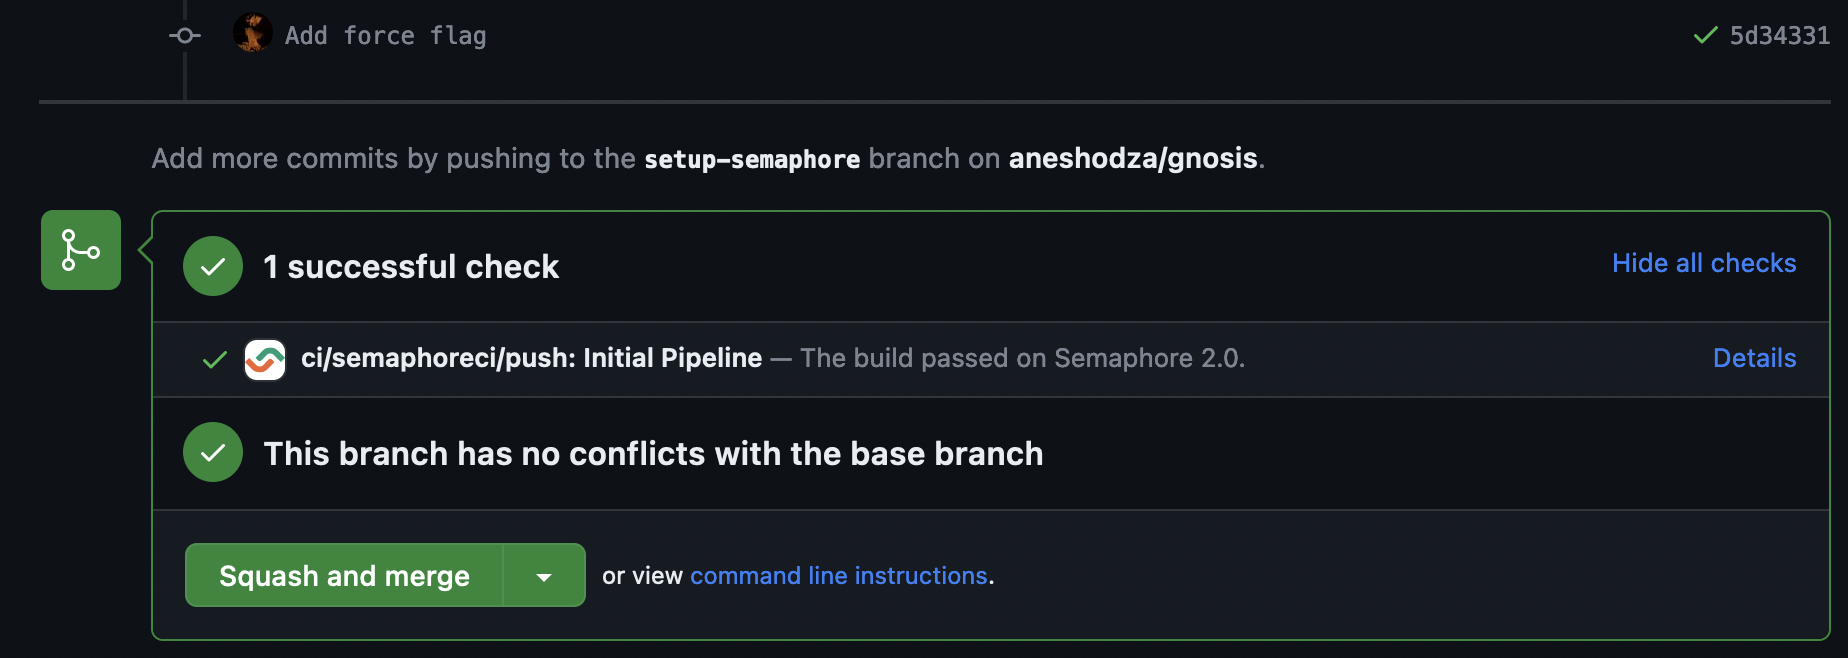
\includegraphics[width=0.8\textwidth]{images/misc/ci-passed.png}
  \caption[Screenshot des GitHub Status Checks, worauf SemaphoreCI sichtbar ist]{GitHub Status Checks mit SemaphoreCI}
  \label{fig:semaphore_ci_passed}
\end{figure}

\subsubsection{SimpleCov}
Um die Test-Coverage zu messen, wird SimpleCov verwendet. SimpleCov ist ein Ruby Gem, welches die Test-Coverage misst und
dann in einem HTML Report ausgibt. Ausserdem kann man eine minimale Test-Coverage definieren, welche beim Unterschreiten
die Tests fehlschlagen lässt. Damit das funktioniert müssen wir SimpleCov einbinden und dann die Dateien, welche wir
auf ihre Test-Coverage prüfen wollen, laden\newline
Die Implementation findet im test\_helper.rb statt und sieht wie folgt aus:
\begin{codebox}[]
  \begin{minted}{ruby}
# frozen_string_literal: true

require 'simplecov'

SimpleCov.coverage_dir('plugins/gnosis/coverage')
SimpleCov.start do
add_filter do |source_file|
  source_file.lines.count < 7
end

add_filter do |source_file|
  source_file.filename.exclude?('gnosis/app')
end
end

SimpleCov.minimum_coverage 100

Dir[Rails.root.join('plugins/gnosis/app/**/*.rb')].each { |f| load f }

# Load the Redmine helper
require File.expand_path("#{File.dirname(__FILE__)}/../../../test/test_helper")
  \end{minted}
\end{codebox}
\textbf{Zu beachten:} Auf Zeile acht wird die mindeste Zeilenanzahl der Dateien auf 7 anstatt 5 gesetzt. Das hat den
Grund, dass Rails Klassen meistens mit einem \bgmintinline{ruby}{# frozen_string_literal: true} gefolgt von einer
leeren Zeile beginnen. Das führt dazu, dass Klassen mit vier Zeilen zu Dateien mit sechs Zeilen werden. Das wurde mit
der VF so abgesprochen. \newline

Wenn wir dann unser Plugin testen, gibt SimpleCov folgenden Report aus:
\begin{codebox}
  \begin{minted}{bash}
Coverage report generated for Minitest to /Users/anes/c/redmine/plugins/gnosis/coverage. 3 / 3 LOC (100.0%) covered.
  \end{minted}
\end{codebox}

\subsubsection{FactoryBot \& Faker}
Damit die Tests mit Beispieldaten arbeiten können, wird FactoryBot in Kombination mit Faker verwendet. FactoryBot ist ein
Rubygem, welcher das Erstellen von Daten vereinfacht. In diesem Fall wird es aber nur für Testdaten genutzt. Um dann die
Attribute zu befüllen wird Faker verwendet. Dieser Rubygem generiert zufällige Daten, wie beispielsweise Namen, Adressen
oder Telefonnummern. \newline
Damit FactoryBot richtig eingebunden wird, muss man test\_helper.rb anpassen:
\begin{codebox}[]
  \begin{minted}{ruby}
FactoryBot.definition_file_paths = [File.expand_path('factories', __dir__)]
FactoryBot.find_definitions
  \end{minted}
\end{codebox}

\subsection{init.rb}
Im init.rb eines Plugins werden allgemeine Daten wie Name, Autor, Version und so weiter definiert. Dieses File sieht
in diesem Fall folgendermassen aus:
\begin{codebox}[]
  \begin{minted}{ruby}
Redmine::Plugin.register :gnosis do
  name 'Gnosis plugin'
  author 'Anes Hodza'
  description 'This Plugin allows you to see the status of issues in a project'
  version '0.0.1'
  url 'https://github.com/aneshodza/gnosis/'
  author_url 'https://www.aneshodza.ch/'
end
  \end{minted}
\end{codebox}

\section{Umsetzung der Datenstruktur}
Da unter Kapitel \ref{sec:decide_erd} die Entscheidung getroffen wurde die \enquote{has many trough} Beziehung zu
verwenden, wird diese auch implementiert. Das bedeutet, dass wir zwei Objekte erstellen müssen: 
\bgmintinline{ruby}{class PullRequest} und \bgmintinline{ruby}{class Deployment}. Diese muss man mit dem Redmine CLI generieren,
damit die neuen Objekte richtig mit den anderen Objekten von Redmine interagieren können. Für das Generieren unserer
Objekte muss man folgende Befehle ausführen:
\begin{codebox}[]
  \begin{minted}{bash}
rails generate redmine_plugin_model gnosis PullRequest 
rails generate redmine_plugin_model gnosis Deployment
rake redmine:plugins:migrate
  \end{minted}
\end{codebox}
\textbf{Wichtig:} Die Migrationen wurden noch mit den Attributen aus dem ERD befüllt. \newline
Um dann die Associations nach Rails Standard zu machen, müssen wir unsere neuen Objekte wie folgt anpassen:
\begin{codebox}[]
  \begin{minted}{ruby}
# app/models/pull_request.rb
class PullRequest < ApplicationRecord
  belongs_to :issue
  has_many :deployments, dependent: :destroy
end

# app/models/deployment.rb
class Deployment < ApplicationRecord
  belongs_to :pull_request
  has_one :issue, through: :pull_request
end

# app/models/gnosis_application_record.rb
class GnosisApplicationRecord < ActiveRecord::Base
  self.abstract_class = true
end
  \end{minted}
\end{codebox}

\section{Daten erstellen und manipulieren}
Damit wir dem Nutzer Daten anzeigen können, müssen wir diese erstellen. Dafür braucht es: einen Listener, welcher auf
die Webhook Events wartet, sowie einen Handler, welcher die Daten verarbeitet und Objekte erstellt. \newline
Dieses Konzept braucht es für GitHub sowie SemaphoreCI.

\subsection{Vorarbeiten}
\label{sec:webhook_prework}
Als Erstes muss ein Controller erstellt werden, in welchem sich beide Listener befinden. Dieser Controller wird wie
folgt erstellt:
\begin{codebox}[]
  \begin{minted}{bash}
bundle exec rails generate redmine_plugin_controller gnosis webhooks
  \end{minted}
\end{codebox}

Dies generiert einen Controller mit dem Namen \bgmintinline{ruby}{WebhooksController}. Da die Webhook Listener als
API Funktionen agieren, müssen wir noch die von Rails eingebaute CSRF Protection deaktivieren. Damit sieht der
Controller so aus:
\begin{codebox}[]
  \begin{minted}{ruby}
class WebhooksController < ApplicationController
  protect_from_forgery except: %i[github_webhook_catcher semaphore_webhook_catcher]
end
  \end{minted}
\end{codebox}

Dann müssen wir die Environment-Keys aufsetzen. Das machen wir, indem wir eine YAML Datei lesen und in eine Konstante
schreiben. Das tun wir wie folgt im \bgmintinline{bash}{init.rb}:
\begin{codebox}[]
  \begin{minted}{ruby}
yaml_data = YAML.safe_load(ERB.new(
  Rails.root.join('plugins/gnosis/config/application.yml').read).result)
ENV = ActiveSupport::HashWithIndifferentAccess.new(yaml_data)
# Rest des init.rb
  \end{minted}
\end{codebox}

\subsection{Pull Request Objekte}
Als Erstes wird der Event Listener für die Pull Request Objekte erstellt, welcher auf die Webhook Events
von GitHub wartet. Wenn ein Event empfangen wird, wird der Handler aufgerufen. Dieser Prozess ist auf dem Deployment
Diagramm unter Kapitel \ref{fig:deployment-diagram} gut ersichtlich. \newline
Die Listener zu Handler Dynamik sieht im Code wie folgt aus:
\begin{codebox}[]
  \begin{minted}{ruby}
# app/controllers/webhooks_controller.rb
class WebhooksController < ApplicationController
  protect_from_forgery except: %i[github_webhook_catcher semaphore_webhook_catcher]

  def github_webhook_catcher
    github_webhook_handler(params)

    render json: {status: :ok}
  end

  def semaphore_webhook_catcher
    semaphore_webhook_handler(params)

    render json: {status: :ok}
  end

  private

  def github_webhook_handler(params)
    numbers = params[:pull_request][:head][:ref].match(%r{/(\d+)})

    if numbers.length.positive? && Issue.exists?(id: numbers[1])
      PullRequest.auto_create_or_update(params.merge(issue_id: numbers[1]))
    end
  end
end
  \end{minted}
\end{codebox}

Um dann die Objekte zu erstellen, muss eine neue Methode erstellt werden, welche die Parameter entgegennimmt und nur
falls nötig ein neues Objekt erstellt. Ausserdem soll der Status auf \enquote{merged} gesetzt werden, falls die Pull
Request bereits gemerged wurde oder auf \enquote{draft}, falls es ein Draft ist. Diese Methode sieht wie folgt aus:
\begin{codebox}[]
  \begin{minted}{ruby}
# app/models/pull_request.rb
class PullRequest < GnosisApplicationRecord
  belongs_to :issue
  has_many :deployments, dependent: :destroy

  def self.auto_create_or_update(params)
    state = params[:pull_request][:merged] ? 'merged' : params[:pull_request][:state]
    state = 'draft' if params[:pull_request][:draft]
    pr = PullRequest.find_or_initialize_by(source_branch: params[:pull_request][:head][:ref])
    pr.update!(state: state, url: params[:pull_request][:html_url],
               title: params[:pull_request][:title], source_branch: params[:pull_request][:head][:ref],
               target_branch: params[:pull_request][:base][:ref], was_merged: params[:pull_request][:merged],
               merge_commit_sha: params[:pull_request][:merge_commit_sha], issue_id: params[:issue_id])
  end
end
  \end{minted}
\end{codebox}
Wenn man diesen Code mit dem Activity Diagramm vergleicht, wird schnell ersichtlich, wie das Activity Diagramm darin
widergespiegelt wird. Hier ist das gleiche Activity Diagramm wie unter Kapitel \ref{fig:activity_hook_call} nochmals,
aber mit Zeilen aus dem Code (Die erste Zahl sagt aus welchem Codeblock die Zeile stammt, die Zweite die Zeilennummer
selbst).
\begin{figure}[H]
  \centering
  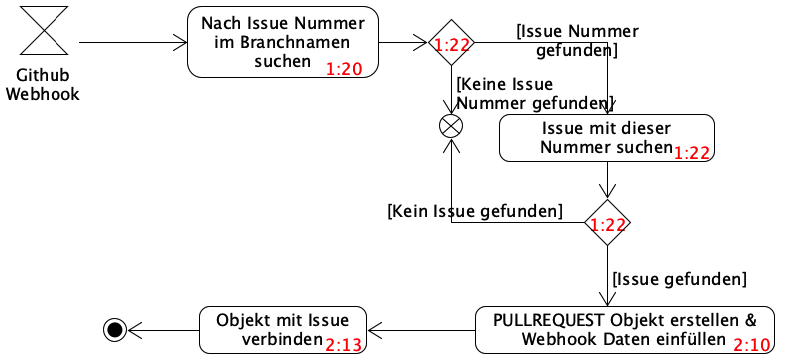
\includegraphics[width=0.8\textwidth]{images/activity/pr_webhook_lines.png}
  \caption[Activity Diagramm zu GitHub Pull Requests Webhook Daten mit Codezeilen]{GitHub Webhook Activity mit Codezeilen}
  \label{fig:activity_diagram_pr_webhook_lines}
\end{figure}

\subsubsection{Webhook Sicherheit}
Unter Kapitel \ref{sec:webhook_prework} wurde die CSRF Protection deaktiviert. Dies ist ein Sicherheitsrisiko, da
jetzt jeder Dritte Daten an das Backend schicken kann. Um dieses Risiko zu minimieren, verwendet GitHub eine Signatur,
welche, ohne jemals den Key zu zeigen, die Daten signiert. Diese Signatur funktioniert nach dem gleichen Prinzip wie
Hashes: Die Daten werden Einweg-Verschlüsselt mit einem geheimen Key. Dann kann im Backend der gleiche Prozess 
durchgeführt werden und die beiden Hashes verglichen werden. Wenn diese übereinstimmen, sind die Daten echt. Dieses
Prinzip wird auch bei Passwörtern genutzt. \cite{password_storage} \newline
Die Implementation sieht wie folgt aus:
\begin{codebox}[]
  \begin{minted}{ruby}
# app/controllers/webhooks_controller.rb
def github_webhook_catcher
  p_body = request.body.read
  unless verify_signature(p_body, request.env['HTTP_X_HUB_SIGNATURE_256'])
    return render json: {status: 403}, status: :forbidden
  end
  # ...
end

private

def verify_signature(payload_body, recieved_signature)
  signature = "sha256=#{OpenSSL::HMAC.hexdigest(OpenSSL::Digest.new('sha256'), ENV.fetch('GITHUB_WEBHOOK_SECRET', 'test'),
                                                payload_body)}"

  Rack::Utils.secure_compare(signature, recieved_signature)
end
  \end{minted}
\end{codebox}

\subsubsection{Webhook Aufsetzen}
Um die Webhook aufzusetzen, begibt man sich auf \url{https://github.com/org/repo/settings/hooks} und klickt auf
\enquote{Add Webhook}. Die Payload url ist \enquote{Deine URL + /github\_webhook}. Der Secret Key ist ein beliebiger
String, welcher im Backend als Umgebungsvariable gesetzt werden muss. Schlussendlich muss man noch die Events
auswählen, welche gesendet werden sollen. In diesem Fall sind dies die \enquote{Pull requests}.
\begin{figure}[H]
  \centering
  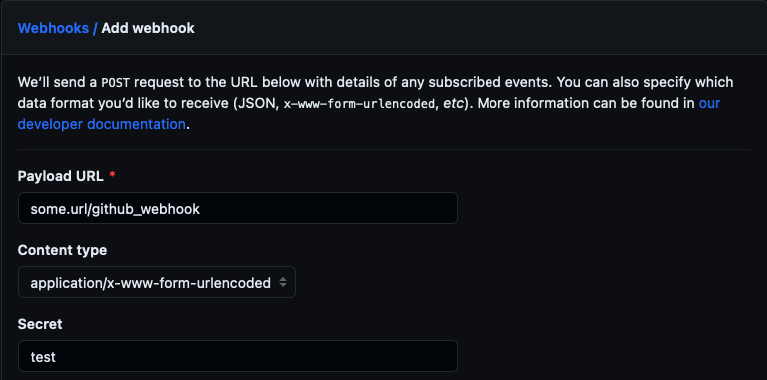
\includegraphics[width=0.8\textwidth]{images/misc/setup_webhook.png}
  \caption[Screenshot vom GitHub Webhook Setup]{GitHub Webhook Setup}
  \label{fig:github_webhook}
\end{figure}

\subsection{Deployment Objekte}
Zunächst wird der Event Listener für die Deployment Objekte erstellt, welcher auf die Webhook Events von Semaphore
wartet. Auch hier wird das gleiche Prinzip wie bei den Pull Requests angewendet. Der Listener kümmert sich um die
Abnahme sowie Verifikation der Request und gibt diese dann an den Handler weiter. \newline
\textbf{Zu beachten:} Plan B wurde verwendet, da die Semaphore Webhooks nicht genug Daten mitschicken. \newline
Auch hier wird die gleiche Listener und Handler Struktur wie bei den Pull Requests verwendet. So sieht die
Implementation aus:
\begin{codebox}[]
  \begin{minted}{ruby}
# app/controllers/webhooks_controller.rb
class WebhooksController < ApplicationController
  # ...
  def semaphore_webhook_catcher
    semaphore_webhook_handler(params)

    render json: {status: :ok}
  end

  private

  def semaphore_webhook_handler(params)
    range = params[:revision][:branch][:commit_range]
    branch = params[:revision][:branch][:name]
    repo = params[:repository][:slug]
    passed = params[:pipeline][:result] == 'passed'
    time = params[:pipeline][:done_at]

    first_sha = range.split('...').first
    last_sha = range.split('...').last

    sha_between = fetch_commit_history(repo, branch, first_sha, last_sha)
    create_deploys_for_pull_requests(sha_between, branch, passed, time)
  end
  # ...
end
  \end{minted}
\end{codebox}
Hier ist viel Code nötig um die Daten zu verarbeiten und die Deployments ihren Pull Requests zuzuordnen. Auf Zeile 19
wird die Commit-History aus dem GitHub geholt. Diese wurde wie folgt implementiert:
\begin{codebox}[]
  \begin{minted}{ruby}
# app/controllers/webhooks_controller.rb
class WebhooksController < ApplicationController
  # ...
  Octokit.configure do |config|
    config.access_token = ENV.fetch('GITHUB_ACCESS_TOKEN', nil)
  end
  CLIENT = Octokit::Client.new
  # ...
  private
  # ...
  def fetch_commit_history(repo, branch, first_commit, last_commit)
    commit_sha_list = CLIENT.commits(repo, branch).pluck(:sha)

    first_commit_index = commit_sha_list.index(first_commit)
    last_commit_index = commit_sha_list.index(last_commit)

    commit_sha_list[last_commit_index..first_commit_index]
  end
  # ...
end
  \end{minted}
\end{codebox}
Dann wird auf Zeile 20 des Ersten Codeblocks die Methode \bgmintinline{ruby}{def create\_deploys\_for\_pull\_requests}
aufgerufen. Diese erstellt alle Deployment Objekte für die Pull Requests, welche in der Commit-History gefunden wurden.
Dafür wird auch wie bei den Pull Requests eine \enquote{intelligente} create Methode erstellt:
\begin{codebox}[]
  \begin{minted}{ruby}
# app/controllers/webhooks_controller.rb
class WebhooksController < ApplicationController
  # ...
  def create_deploys_for_pull_requests(sha_list, branch, passed, ci_date_string)
    sha_list.each do |sha|
      pull_request = PullRequest.find_by(sha: sha)
      next unless pull_request

      Deployment.auto_create_or_update(branch, pr.id, url, passed, ci_date_string)
    end
  end

  def url
    "https://#{params[:organization][:name]}
      .semaphoreci.com/workflows/#{params[:workflow][:id]}/"
  end
  # ...
end

# app/models/deployment.rb
class Deployment < GnosisApplicationRecord
  # ...
  def self.auto_create_or_update(branch, pull_request_id, url, has_passed, ci_date_string)
    ci_date = Time.zone.parse(ci_date_string)
    deploy = Deployment.find_or_initialize_by(deploy_branch: branch, pull_request_id: pull_request_id, ci_date: ci_date_string)
    deploy.update!(url: url, has_passed: has_passed)
  end
end
  \end{minted}
\end{codebox}
Auch hier schlägt die Implementation klare Brücken zu den Activity-Diagrammen. In folgender Grafik ist das
Activity-Diagramm aus Kapitel \ref{fig:activity_plan_b} mit Code Zeilen notiert. Die erste Zahl ist der Codeblock und
die Zweite die Zeile.
\begin{figure}[H]
  \centering
  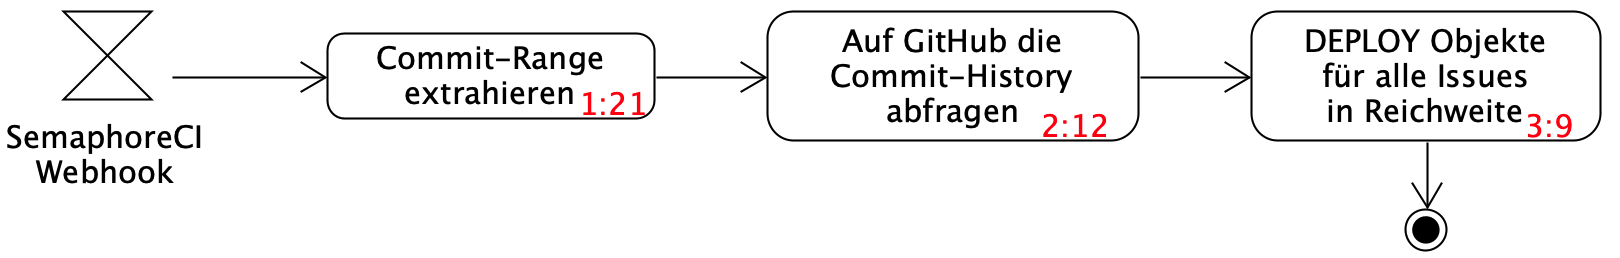
\includegraphics[width=0.8\textwidth]{images/activity/plan_b_code.png}
  \caption[Activity Diagramm zu SemaphoreCI Webhook Daten mit Codezeilen]{SemaphoreCI Webhook Activity mit Codezeilen}
  \label{fig:activity_plan_b_code}
\end{figure}

\subsubsection{Webhook Sicherheit}
Die Sicherheit der Semaphore Webhooks läuft gleich wie die von GitHub ab: Es wird ein Secret Key verwendet,
welcher vom Dienst mithilfe von HMAC-SHA256 signiert wird. Dieser wird dann im Header mitgeschickt. Somit erhaltet
das Backend eine Signatur, welche mit dem Secret Key verifiziert werden kann. \newline
Die Implementation sieht wie folgt aus:
\begin{codebox}[]
  \begin{minted}{ruby}
# app/controllers/webhooks_controller.rb
def semaphore_webhook_catcher
  unless verify_signature(request.body.read, "sha256=#{request.headers['X-Semaphore-Signature-256']}",
                          ENV.fetch('SEMAPHORE_WEBHOOK_SECRET', nil))
    return render json: {status: 403}, status: :forbidden
  end

  semaphore_webhook_handler(params)

  render json: {status: :ok}
end
  \end{minted}
\end{codebox}
Es wird die gleiche \bgmintinline{ruby}{def verify_signature} Methode wie zuvor verwendet. Nur die Parameter
unterscheiden sich leicht.

\subsubsection{Aufsetzen der Webhook}
Hierfür begibt man sich auf \url{https://deine_organisation.semaphoreci.com/notifications} und klickt auf 
\enquote{New Notification}. Attribute wie \enquote{Name of the notification}, \enquote{Name of the rule} und so weiter
sind selbst zu entscheiden. Wichtig ist, dass man die Projekte unter \enquote{In Projects} auflistet, unter 
\enquote{Pipelines} den Regex String \bgmintinline{bash}{/.*-deploy\.yml/} einträgt und zum Schluss unter Webhook
seine URL + /semaphore\_webhook, sowie WEBHOOK\_SECRET unter \enquote{Secret Name} einträgt. \newline
Danach muss die Signatur aufgesetzt werden. Dafür geht man unter
\url{https://deine_organisation.semaphoreci.com/secrets} und klickt auf \enquote{New Secret}. Das wird WEBHOOK\_SECRET
benannt und der Wert ist der Secret Key.
\begin{figure}[H]
  \centering
  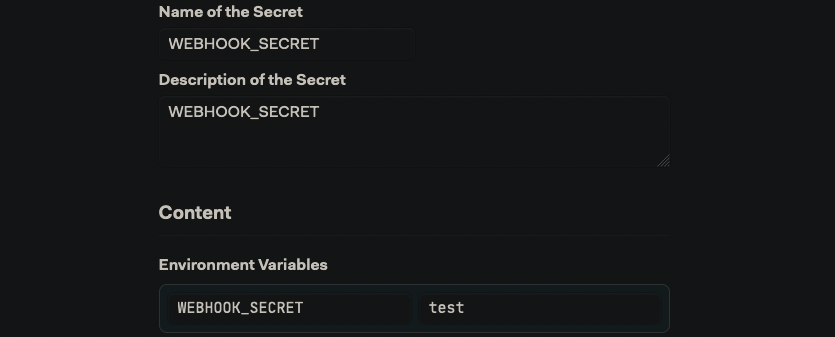
\includegraphics[width=0.8\textwidth]{images/misc/setup_semaphore_webhook.png}
  \caption[Screenshot des Setups des SemaphoreCI Secret Key]{Setup des SemaphoreCI Secret Key}
  \label{fig:setup_semaphore_webhook}
\end{figure}

\subsection{Wieso aktiv Gepollt wird}
\label{sec:why_active_polling}
Obwohl Software-Design Anforderung 5 besagt, dass aktives Polling der Dienste nicht vorkommen sollte, ist
es bei guter Begründung erlaubt. In diesem Fall wird aktiv GitHub abgefragt, weil die Informationen von
den SemaphoreCI Webhooks nicht ausreichen. Diese geben nämlich eine \enquote{Commit-Range} an, anstatt
eine Liste aller Commits, welche soeben released wurden. \newline
Falls das Plugin alle GitHub Pull Requests richtig abfangen würde, dürfte das eigentlich kein Problem sein,
doch das würde zu einem \enquote{Single Point of failure} führen. Falls nur schon eine Pull Request verpasst
wird, kann es sein, dass diese direkt am Rand der \enquote{Commit-Range} liegt und somit die Range nicht
eingegrenzt werden kann. Das sieht ungefähr so aus:
\begin{figure}[H]
  \centering
  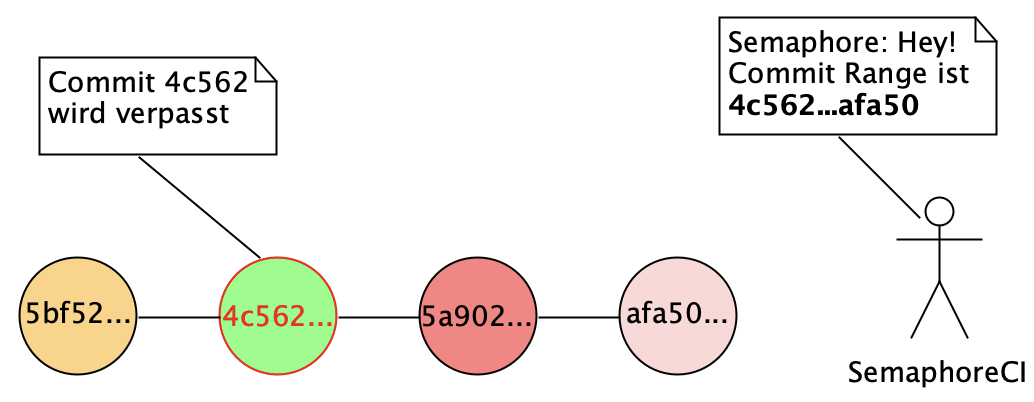
\includegraphics[width=0.8\textwidth]{images/misc/missed_commit_range.png}
  \caption[UMLet Diagramm eines Beispiels für verpasste Commits]{Beispiel für verpasste Commits}
  \label{fig:commit_range}
\end{figure}
Falls aber der erste Commit in der Range fehlt, ist das eher weniger ein Problem, da man nachschauen
kann, welcher der erste, noch nicht releaste, Commit ist und dann die Range manuell eingrenzen kann. \newline
Falls aber der letzte fehlt, kann man das nicht mehr. Und was passiert, falls die History Rebased wird?
Und in anderen Edge-Cases? Falls diese PA ein Produkt liefern will, welches in der Praxis eingesetzt wird,
liefert das aktive Polling eine zusätzliche Schicht Sicherheit, dass die kommunizierten Daten wahrheitsgetreu
sind.

\subsection{GitHub Token}
Damit das Plugin die GitHub Repositories abfragen kann, muss es sich authentifizieren. Dafür wird ein GitHub
Token verwendet. Dieses wird im \bgmintinline{bash}{application.yml} als GITHUB\_ACCESS\_TOKEN gespeichert.
\newline
Um das Token zu erstellen, begibt man sich auf \url{https://github.com/settings/tokens} und klickt auf
\enquote{Generate new Token} und wählt die \enquote{(classic)} Version aus. Danach gibt man dem Token Zugriff
auf \enquote{repo}, was bereits reichen sollte.
\begin{figure}[H]
  \centering
  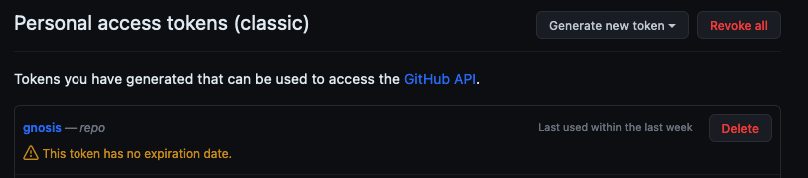
\includegraphics[width=0.8\textwidth]{images/misc/github-access-token.png}
  \caption[Screenshot des GitHub Access Tokens]{GitHub Access Token}
  \label{fig:setup_github_token}
\end{figure}

\section{Erstellen der Views}
Um die Implementation zu vervollständigen, müssen noch die Views erstellt werden. Für diese besteht bereits ein
Mockup (Abbildung \ref{fig:mockup_sublists}).
\subsection{Aufsetzen der Hook}
Da die View dieser PA nicht auf einer eigenen Seite, sondern unter Issue Details angezeigt wird, kann man nicht
einfach einen Controller erstellen, welcher die View zurückschickt. Es wird ein von Redmine eingebautes Feature
verwendet: Hooks \cite{redmine_hooks}. \newline
Dafür geht man als erstes in den \bgmintinline{bash}{/lib/} Ordner und erstellt die Hook Datei. In diesem Fall wurde
diese \bgmintinline{bash}{issue_details_hook_listener.rb} benannt. In diese wird die (von Redmine gegebene)
\bgmintinline{ruby}{def view_issues_show_description_bottom} Methode implementiert. Das sieht wie folgt aus:
\begin{codebox}[]
  \begin{minted}{ruby}
class NewSectionHookListener < Redmine::Hook::ViewListener
  def view_issues_show_description_bottom(context={})
  end
end
  \end{minted}
\end{codebox}
Der Parameter \bgmintinline{ruby}{context={}} enthält wichtige Informationen zum Kontext in welchem die View 
angefragt wurde. In diesem Fall sind das beispielsweise das Issue, Projekt und so weiter. \newline
\subsection{Laden der Daten}
Als Nächstes werden die Daten aus der Datenbank geladen. Für diesen Call müssen alle Pull Requests, welche
zu diesem Issue gehören, sowie dessen Deployments abgefragt werden. \newline
Die Pull Requests können mit \bgmintinline{ruby}{@prs = PullRequest.where(issue_id: @context[:issue].id).to_a}
per ORM geholt werden. Dessen Deployments widerrum dann mit
\bgmintinline{ruby}{@deployments = @prs.map { |pr| Deployment.where(pull_request_id: pr['id']).to_a } }. \newline
\subsection{Rendern der View}
Die View selbst ist der Return Value der \bgmintinline{ruby}{def view_issues_show_description_bottom} Methode. Dieser
muss in Form eines Strings zurückgegeben werden, welcher dann als HTML interpretiert wird. \newline
Das bedeutet, dass das HTML für die View im Backend in Ruby Code geschrieben werden muss. Als Erstes braucht es das
Grundgerüst der View. Dieses sieht wie folgt aus:
\begin{codebox}[]
  \begin{minted}{ruby}
# lib/new_section_hook_listener.rb
class NewSectionHookListener < Redmine::Hook::ViewListener
  def view_issues_show_description_bottom(context={})
    @context = context
    setup
    <<-HTML
      <hr/>
      <p><strong>Pull Requests</strong></p>
      #{@pr_string.length.positive? ? "<ul>#{@pr_string}</ul>" :
        'There are currently no PRs open for this issue'}
    HTML
  end
end
  \end{minted}
\end{codebox}
Diese Funktion kümmert sich um das Rendern des HTMLs, sowie das anzeigen der richtigen Nachricht, falls keine Daten
da sind. Damit aber \bgmintinline{ruby}{@pr_string} Daten enthält, gibt es die \bgmintinline{ruby}{setup} Methode.
Diese Sammelt alle Daten und speichert diese in Instanz Methoden, damit nicht alles per Parameter übergeben werden
muss. Diese sieht wie folgt aus:
\begin{codebox}[]
  \begin{minted}{ruby}
# lib/new_section_hook_listener.rb
class NewSectionHookListener < Redmine::Hook::ViewListener
  #...
  private

  def setup
    get_prs
    get_deployments
    set_deployment_strings
    set_pr_string
  end
end
  \end{minted}
\end{codebox}
Die \bgmintinline{ruby}{def get_prs} sowie \bgmintinline{ruby}{def get_deployments} kümmern sich beide um das Laden
von Pull Requests und dessen Deployments, wie oben erklärt. Diese wurden wie folgt implementiert:
\begin{codebox}[]
  \begin{minted}{ruby}
# lib/new_section_hook_listener.rb
class NewSectionHookListener < Redmine::Hook::ViewListener
  #...
  private
  #...
  def get_prs
    @prs = PullRequest.where(issue_id: @context[:issue].id).to_a
  end

  def get_deployments
    @deployments = @prs.map do |pr|
      Deployment.where(pull_request_id: pr['id']).to_a
    end
  end
end
  \end{minted}
\end{codebox}
Zum Schluss müssen noch die Daten schön formatiert werden. Darum kümmern sich die \newline
\bgmintinline{ruby}{def set_deployment_strings} und \bgmintinline{ruby}{def set_pr_string} Methoden. Diese wurden
wie folgt implementiert:
\begin{codebox}[]
  \begin{minted}{ruby}
# lib/new_section_hook_listener.rb
class NewSectionHookListener < Redmine::Hook::ViewListener
  #...
  private
  #...
  def set_deployment_strings
    @deployments_strings = []
    @deployments.each do |deployment_list|
      formatted_deployment_list = []
      deployment_list.each do |deployment|
        formatted_deployment_list << <<-LISTOBJECT
          <li>
            <a href='#{deployment['url']}' target='_blank'
              id='deployment-#{deployment['id']}'>
                on "#{deployment['deploy_branch']}"
                at #{deployment['ci_date'].strftime('%d.%m.%Y at %I:%M%p UTC')}
                #{deployment['has_passed'] ? 'p' : 'x'} 
              </a>
          </li>
        LISTOBJECT
      end
      @deployments_strings << formatted_deployment_list
    end
  end

  def set_pr_string
    @pr_string = @prs.each_with_index.map do |pr, index|
      formatted_deployments_list = @deployments_strings[index].join
      <<-LISTOBJECT
      <li>
        <a href='#{pr['url']}' target='_blank'
          id='pr-#{pr['id']}'>#{pr['title']} (#{pr['state']})</a>
        <ul>
          #{formatted_deployments_list}
        </ul>  
      </li>
      LISTOBJECT
    end.join
  end
end
  \end{minted}
\end{codebox}
\subsection{Registrieren der Hook}
Damit die View angezeigt wird, muss die Hook noch in der \bgmintinline{bash}{init.rb} Datei registriert werden. Das
kann man einfach mit einem \bgmintinline{ruby}{require} machen. Das \bgmintinline{bash}{init.rb} sieht dann wie folgt aus:
\begin{codebox}[]
  \begin{minted}{ruby}
# init.rb
require 'redmine'
require_relative 'lib/issue_details_hook_listener'
  \end{minted}
\end{codebox}
\subsection{Resultat}
Diese Komponenten zusammen ergeben dann folgende View:
\begin{figure}[H]
  \centering
  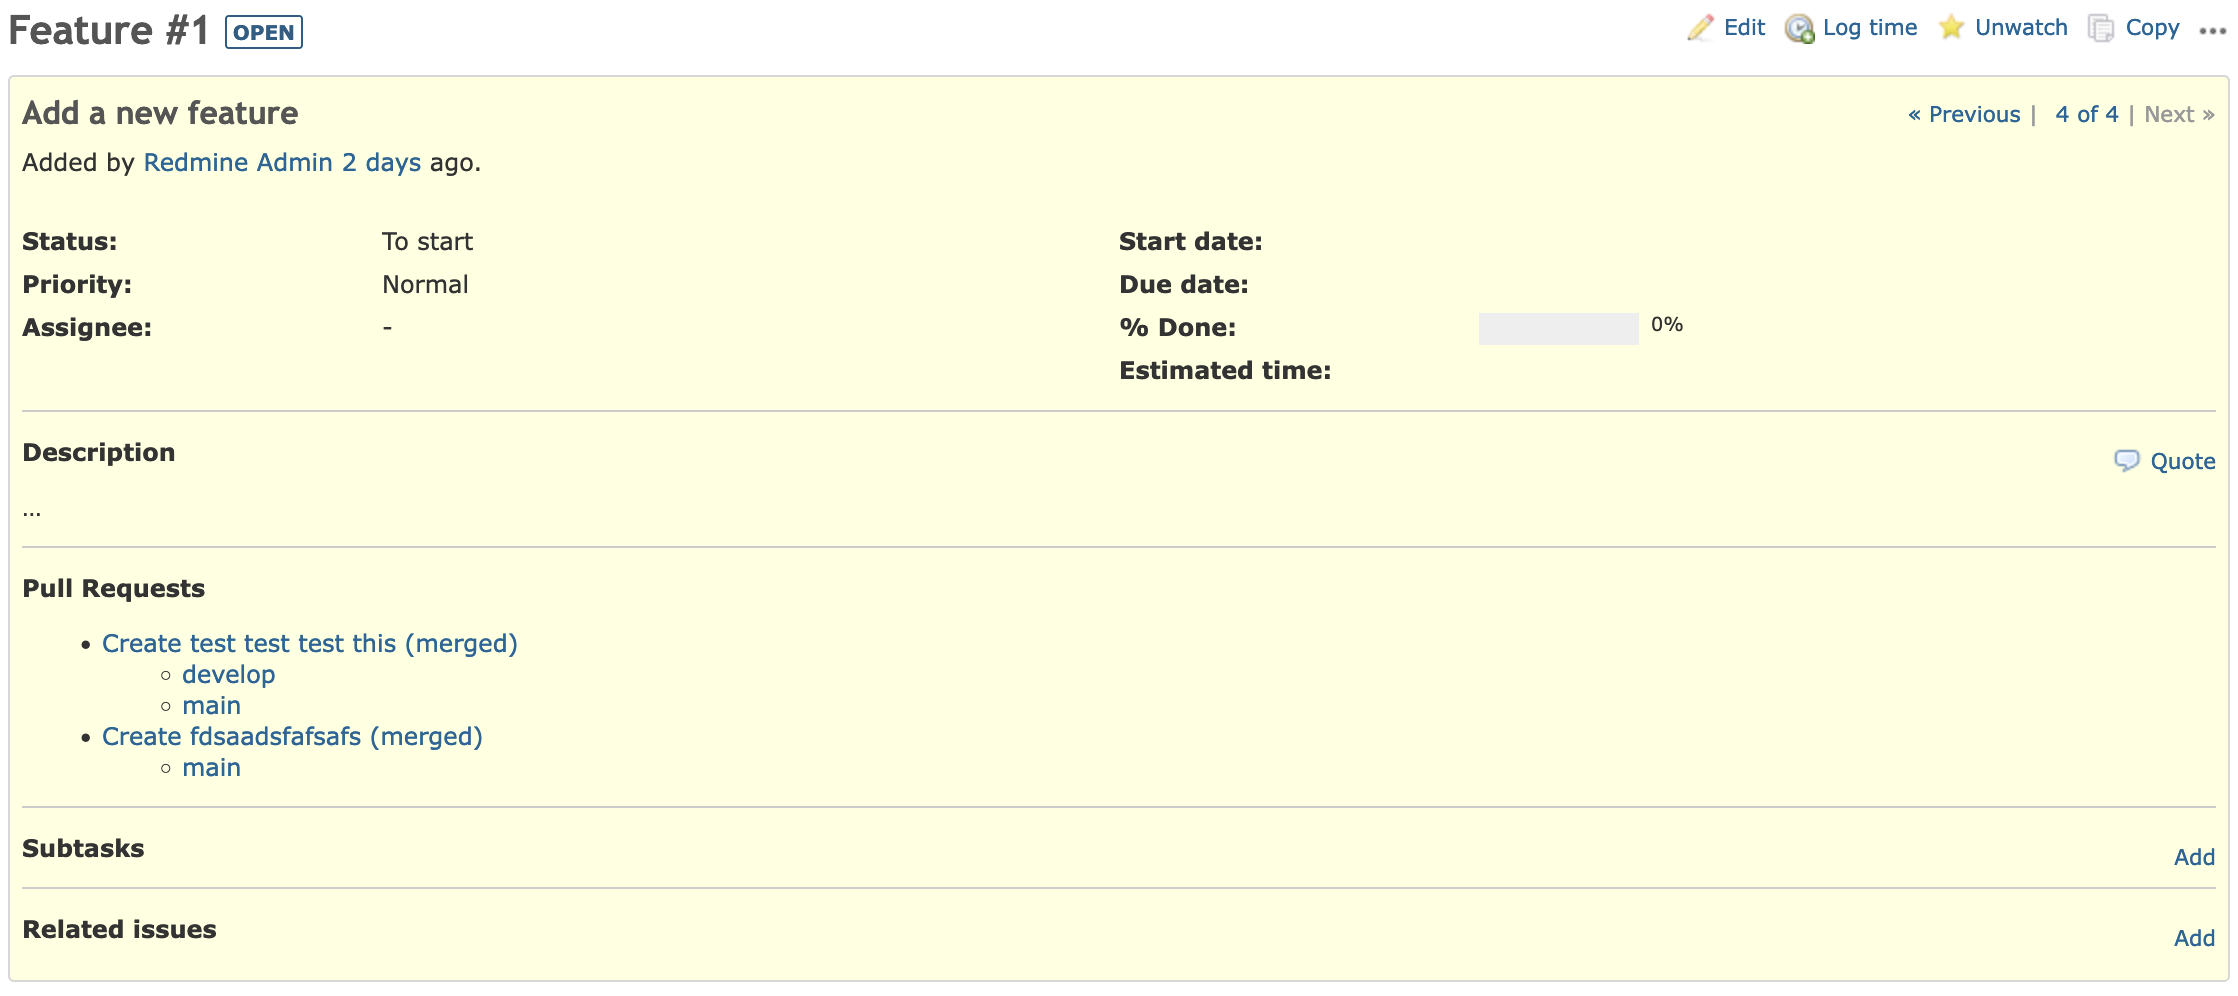
\includegraphics[width=0.8\textwidth]{images/misc/issue_details.png}
  \caption[Screenshot eines Issues mit ausgebauter View]{Issue mit ausgebauter View}
  \label{fig:issue_details}
\end{figure}
